\documentclass[10pt]{exam}

\usepackage{amssymb, amsmath, amsthm, mathrsfs, multicol, graphicx} 
\usepackage{tikz}

\def\d{\displaystyle}
\def\?{\reflectbox{?}}
\def\b#1{\mathbf{#1}}
\def\f#1{\mathfrak #1}
\def\c#1{\mathcal #1}
\def\s#1{\mathscr #1}
\def\r#1{\mathrm{#1}}
\def\N{\mathbb N}
\def\Z{\mathbb Z}
\def\Q{\mathbb Q}
\def\R{\mathbb R}
\def\C{\mathbb C}
\def\F{\mathbb F}
\def\A{\mathbb A}
\def\X{\mathbb X}
\def\E{\mathbb E}
\def\O{\mathbb O}
\def\pow{\mathscr P}
\def\inv{^{-1}}
\def\nrml{\triangleleft}
\def\st{:}
\def\~{\widetilde}
\def\rem{\mathcal R}
\def\iff{\leftrightarrow}
\def\Iff{\Leftrightarrow}
\def\and{\wedge}
\def\And{\bigwedge}
\def\AAnd{\d\bigwedge\mkern-18mu\bigwedge}
\def\Vee{\bigvee}
\def\VVee{\d\Vee\mkern-18mu\Vee}
\def\imp{\rightarrow}
\def\Imp{\Rightarrow}
\def\Fi{\Leftarrow}

\def\={\equiv}
\def\var{\mbox{var}}
\def\mod{\mbox{Mod}}
\def\Th{\mbox{Th}}
\def\sat{\mbox{Sat}}
\def\con{\mbox{Con}}
\def\bmodels{=\joinrel\mathrel|}
\def\iffmodels{\bmodels\models}
\def\dbland{\bigwedge \!\!\bigwedge}
\def\dom{\mbox{dom}}
\def\rng{\mbox{range}}
\DeclareMathOperator{\wgt}{wgt}

\def\circleA{(-.5,0) circle (1)}
\def\circleAlabel{(-1.5,.6) node[above]{$A$}}
\def\circleB{(.5,0) circle (1)}
\def\circleBlabel{(1.5,.6) node[above]{$B$}}
\def\circleC{(0,-1) circle (1)}
\def\circleClabel{(.5,-2) node[right]{$C$}}
\def\twosetbox{(-2,-1.5) rectangle (2,1.5)}
\def\threesetbox{(-2,-2.5) rectangle (2,1.5)}


\def\bar{\overline}

%\pointname{pts}
\pointsinmargin
\marginpointname{pts}
\marginbonuspointname{pts-bns}
\addpoints
\pagestyle{head}
%\printanswers

\firstpageheader{Math 228}{\bf Homework 4}{Due: Wed, Feb 13}

\def\vertexsize{4pt}
\newcommand{\vtx}[2]{node[fill,circle,inner sep=0pt, minimum size=\vertexsize,label=#1:#2]{}}
\newcommand{\va}[1]{\vtx{above}{#1}}
\newcommand{\vb}[1]{\vtx{below}{#1}}
\newcommand{\vr}[1]{\vtx{right}{#1}}
\newcommand{\vl}[1]{\vtx{left}{#1}}
\renewcommand{\v}{\vtx{above}{}}

\begin{document}
\noindent \textbf{Instructions}: Same rules as usual - turn in your work on separate sheets of paper.  You must justify all your answers for full credit.

\begin{questions}

\question Edward A. Mouse has just finished his brand new house.  The floor plan is shown below:

\begin{center}
  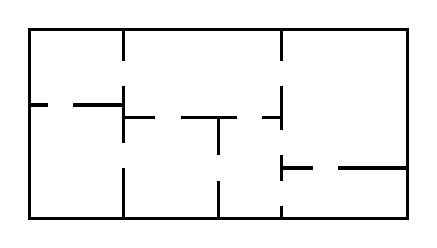
\begin{tikzpicture}[scale=.8]
    \draw[very thick] (-3,0) rectangle (3,3);
    \draw[very thick] (-3,1.8) --(-2.7,1.8) (-2.3,1.8) -- (-1.5, 1.8) (-1.5, 1.6) -- (-1,1.6) (-.6, 1.6) -- (.3,1.6) (.7,1.6) -- (1, 1.6) (1, .8) -- (1.5, .8) (1.9,.8) -- (3,.8); 
    \draw[very thick] (-1.5,0) -- (-1.5, .8) (-1.5, 1.2) -- (-1.5,2.1) (-1.5,2.5) -- (-1.5,3);
    \draw[very thick] (0,0) -- (0,.6) (0,1) -- (0,1.6);
    \draw[very thick] (1,0) -- (1,.2) (1,.6) -- (1,1) (1,1.4) -- (1,2.1) (1,2.5) -- (1,3);
  \end{tikzpicture}
\end{center}


\begin{parts}
 \part[3] Edward wants to give a tour of his new pad to a lady-mouse-friend.  Is it possible for them to walk through every doorway exactly once?  If so, in which rooms must they begin and end the tour? Explain.
 \begin{solution}
   Yes, he must start in the top right room and end in the bottom middle room, or vice versa.  This is because those are the two rooms with an odd number of doors.  
   
   In graph theory terms, if we place a vertex in each room and connect vertices if there is a door between their rooms, we are asking whether the graph has an Euler path.  The number of doors is the degree of the vertex, and a graph has an Euler path if and only if there are two or fewer vertices with odd degree.  In that case, the path must start at one of those odd degree vertices and end at the other.
 \end{solution}

\part[2] Is it possible to tour the house visiting each room exactly once?  Explain.

\begin{solution}
  Yes.  This does not correspond to an Euler path or circuit, since all we need to do is visit each vertex exactly once.  It is easy to do - for example, tour the house clockwise.
\end{solution}


\part[3] After a few mouse-years, Edward decides to remodel.  He would like to add some new doors between the rooms he has.  Of course, he cannot add any doors to the exterior of the house.  Is it possible for each room to have an odd number of doors? Explain.
\begin{solution}
  No it is not possible.  If each room had an odd number of doors, then the corresponding graph would have the property that the degree of every vertex would be odd.  There are 7 vertices, and if their degrees were all odd, then the sum of the degrees would be an odd number as well.  But the number of edges in a graph is always 1/2 the sum of the degrees, so the sum of the degrees must be even.
  
  In other words, if you add up the number of doors in all rooms, you need to get an even number, since the number of doorways is half this number - each doorway counts as a door in two rooms.
\end{solution}

\end{parts}


\question[4] Suppose you are at a party with 19 of your closest friends (so including you, there are 20 people there).  Explain why there must be least two people at the party who are friends with the same number of people at the party.  Assume friendship is always reciprocated.

\begin{solution}
  Suppose this was not the case.  That is, suppose everyone at the party had a {\em different} number of friends.  What could these numbers be.  The would have to be less than 20, so each number from 0 to 19 (that's 20 numbers) must be used exactly once.  But this is impossible. If someone is friends with 19 people, then she is friends with everyone, including the person who is supposedly friends with 0 people.
  
  What this says is that in any simple graph with 20 vertices, there must be at least two vertices which have the same degree.
\end{solution}


\question[4] Prove that the {\em Petersen graph} (below) is not planar.  Hint: what is the length of the shortest circuit?

\begin{center}
  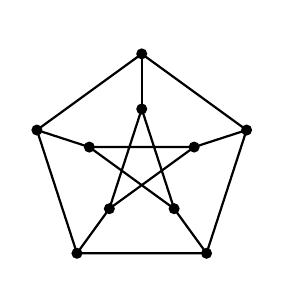
\begin{tikzpicture}[scale=.7]
    \draw[thick] (18:2) -- (90:2) -- (162:2)  -- (234:2) -- (306:2) -- cycle; 
    \draw[thick] (18:1) --  (162:1)  -- (306:1) -- (90:1) -- (234:1) --cycle;
    \foreach \x in {18, 90, 162, 234, 306}
    \draw[thick] (\x:1) \v -- (\x:2) \v;
  \end{tikzpicture}
\end{center}

\begin{solution}
  \begin{proof}
    Suppose, for contradiction, that the Petersen graph were planar.  Then it would satisfy Euler's formula: $V - E + F = 2$.  Since the graph has 10 vertices and 15 edges, this says that there must be $7$ faces.  
    
    Now let $B$ be the total number of boundaries around all faces when the graph is drawn in a planar way.  Since each edge is used in two boundaries we have $B = 2E$.  On the other hand, each face is surrounded by {\em at least} 5 boundaries, since the shortest cycle (circuit) in the graph contains 5 edges.  Thus $B \ge 5F$.  Putting these two facts together we get
    \[5F \le 2E\]
    This is a contradiction, since $5\cdot 7 \not\le 2\cdot 15$.  Alternatively, the above relationship says that $F \le 6$, but we said $F = 7$ above.
    
    Therefore the Petersen graph is not planar.
  \end{proof}

\end{solution}


\question A group of 10 friends decides to head up to a cabin in the woods (where nothing could possibly go wrong).  Unfortunately, a number of these friends have dated each other in the past, and things are still a little awkward.  To get the cabin, they need to divide up into some number of cars, and no two people who dated should be in the same car.
\begin{parts}
  \part[3] What is the smallest number of cars you need if all the relationships were strictly heterosexual?  Represent an example of such a situation with a graph.  What kind of graph do you get?
  \begin{solution}
    2 cars are needed.  Since no boys dated boys and no girls dated girls, it is possible to separate the youths into cars by gender.  The corresponding graph (with vertices representing people and edges representing the fact that those people dated) would be bipartite - there are no edges between two boys and no edges between two girls.  
  \end{solution}

  \part[3] What is the smallest number of cars you need if the relationships could be represented by the Petersen graph (above)?  Assume each person is represented by a vertex, and two people have dated if there is an edge between their vertices. Explain.
  
  \begin{solution}
    3 cars are needed.  The Petersen graph is not bipartite, so 2 cars is not enough.  You can see this because there is an odd circuit.  It is not too difficult to assign vertices to cars (i.e., color the vertices) so that no two adjacent vertices are assigned the same car (color).    
  \end{solution}

  \part[2] What do these questions have to do with coloring? 
  \begin{solution}
    We are really asking for the chromatic number of the graphs.  The smallest number of cars needed is the smallest number of colors needed for a proper vertex coloring.
  \end{solution}

\end{parts}

\question[6] We say that a graph has a {\em Hamilton path} if there is a path which visits each vertex exactly once (you do not need to use every edge in the path).  
\begin{parts}
  \part Suppose a graph has a Hamilton path.  What is the maximum number of vertices of degree one the graph can have?  Explain why your answer is correct.

  \begin{solution}
    Note that a vertex of degree one can only be the start or the end of a Hamilton path - if we go {\em to} a vertex of degree one, we are stuck there - we cannot use the same edge to leave the vertex, because doing so would bring us back to a vertex we have already visited.  If a graph has a Hamilton path, it might start at a vertex of degree one, end at a vertex of degree one, but there cannot be any other vertices of degree one.  Therefore a graph with a Hamilton path can have at most two vertices of degree one.
  \end{solution}

  \part Find a graph which does not have a Hamilton path even though no vertex has degree one.  Explain why your example works.
  
  \begin{solution}
    There are many such graphs.  Here are two examples:
    
    \begin{center}
      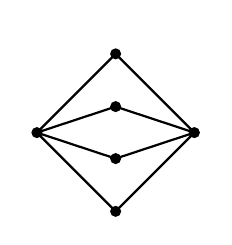
\begin{tikzpicture}
        \draw[thick] (-1,0) \v -- (0,1) \v -- (1, 0) \v -- (0, .33) \v -- (-1,0) -- (0,-.33) \v -- (1,0) -- (0,-1) \v -- (-1,0);
      \end{tikzpicture}
      \hspace{1in}
      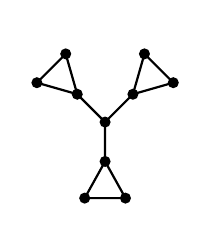
\begin{tikzpicture}
        \draw[thick] (270:.5) \v -- (255:1) \v -- (285:1) \v -- (270:.5) -- (0,0) \v -- (135:.5) \v -- (150:1) \v -- (120:1) \v -- (135:.5) (0,0) -- (45:.5) \v -- (60:1) \v -- (30:1) \v -- (45:.5);
      \end{tikzpicture}

    \end{center}

  \end{solution}

\end{parts}


\end{questions}




\end{document}


